\documentclass[]{standalone}

\usepackage{amsmath}            % \text command
\usepackage{tikz}
\usetikzlibrary{calc}  % coordinate calculations
\usetikzlibrary{arrows}
\usetikzlibrary{positioning} % right = of [something]
\usetikzlibrary{shapes} % rounded rectangle
% \usetikzlibrary{graphs} % graph
\usetikzlibrary{decorations.pathreplacing} % brace
% math
\usepackage{bm, txfonts}
\newcommand{\mc}[1]{\varmathbb{#1}}
\newcommand{\mat}[1]{\bm{#1}}
\renewcommand*{\vec}[1]{\bm{#1}}

\begin{document}

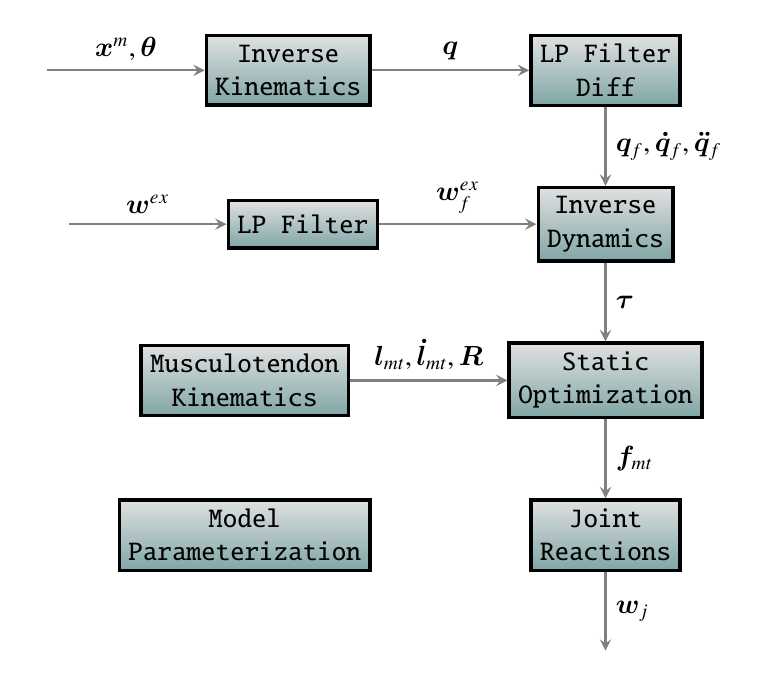
\begin{tikzpicture}[node distance = 1.cm and 2cm,
  terminal/.style={
    % The shape:
    rounded rectangle,
    minimum size=6mm,
    % The rest
    very thick,draw=black!50,
    top color=white,bottom color=black!20,
    font=\ttfamily},
  nonterminal/.style={
    % The shape:
    rectangle,
    % The size:
    minimum size=6mm,
    % The border:
    very thick,
    draw=black!100,
    % The filling:
    top color=gray!80!black!20,
    % a shading that is gray at the top...
    bottom color=cyan!30!black!50, % and something else at the bottom
    % Font
    font=\ttfamily, % \itshape,
    align = center % required if you use new line
  },
  >=stealth, thick, black!50, text=black]

  \node (mocap) {};
  \node (ik) [nonterminal, right = of mocap] {Inverse\\ Kinematics};
  \draw[->] (mocap) -- node [midway, above]{$\vec{x}^m, \vec{\theta}$} (ik);

  \node (ik_filter) [nonterminal, right = of ik] {LP Filter\\ Diff};
  \draw[->] (ik) -- node [midway, above]{$\vec{q}$} (ik_filter);

  \node (id) [nonterminal, below = of ik_filter] {Inverse\\ Dynamics};
  \node (grf_filter) [nonterminal, left = of id] {LP Filter};
  \node (grf) [left = of grf_filter] {};

  \draw[->] (grf) -- node [midway, above]{$\vec{w}^{ex}$} (grf_filter);
  \draw[->] (grf_filter) -- node [midway, above]{$\vec{w}_f^{ex}$} (id);
  \draw[->] (ik_filter) -- node [midway, right]{$\vec{q}_f, \vec{\dot{q}}_f, \vec{\ddot{q}}_f$} (id);

  \node (so) [nonterminal, below = of id] {Static\\ Optimization};
  % \node (emg_filter) [nonterminal, left = of so] {BP, LP\\ Filter};
  % \node (emg) [left = of emg_filter] {};
  \node (mtk) [nonterminal, left = of so] {Musculotendon\\ Kinematics};

  % \draw[->] (emg) -- node [midway, above]{$\vec{e}$} (emg_filter);
  % \draw[->] (emg_filter) -- node [midway, above]{$\vec{e}_f$} (so);
  \draw[->] (id) -- node [midway, right]{$\vec{\tau}$} (so);
  % \draw[->] (ik_filter) -| node [above]{$\vec{q}_f, \vec{\dot{q}}_f, \vec{\ddot{q}}_f$} (mtk);
  \draw[->] (mtk) -- node [midway, above]{$\vec{l}_{mt}, \vec{\dot{l}}_{mt}, \mat{R}$} (so);

  \node (jr) [nonterminal, below = of so] {Joint\\ Reactions};
  \node (jrf) [below = of jr] {};

  \draw[->] (so) -- node [midway, right]{$\vec{f}_{mt}$} (jr);
  \draw[->] (jr) -- node [midway, right]{$\vec{w}_{j}$} (jrf);

  \node (scale) [nonterminal, left = of jr] {Model\\ Parameterization};
\end{tikzpicture}

\end{document}

%%% Local Variables:
%%% mode: latex
%%% TeX-master: t
%%% End: